\documentclass[hyp]{socreport}
\usepackage{fullpage}
\usepackage{color}
\usepackage{listings}
\usepackage{pgfplots}
\lstset{ %
language=C++,                % choose the language of the code
basicstyle=\footnotesize,       % the size of the fonts that are used for the code
backgroundcolor=\color{white},  % choose the background color. You must add \usepackage{color}
showspaces=false,               % show spaces adding particular underscores
showstringspaces=false,         % underline spaces within strings
showtabs=false,                 % show tabs within strings adding particular underscores
frame=single,           % adds a frame around the code
tabsize=2,          % sets default tabsize to 2 spaces
captionpos=b,           % sets the caption-position to bottom
breaklines=true,        % sets automatic line breaking
breakatwhitespace=false,    % sets if automatic breaks should only happen at whitespace
escapeinside={\%*}{*)}          % if you want to add a comment within your code
}

\begin{document}
\pagenumbering{roman}
\title{Mining Definition of Term in Scientific Articles}
\author{Jin Yiping}
\projyear{2012/13}
\projnumber{H079850}
\supervisor{A/P Kan Min-Yen}
\advisor{Ng Jun Ping, He Xiangnan}
\deliverables{
	\item Report: 1 Volume
	\item Source Code: 1 DVD}
\maketitle
\begin{abstract}
In scholarly digital libraries, there are often definitions of key terms in paper articles. In this project, we build a glossary of terms over many thousands of individual research articles. Unlike previous approaches, we define the task of definition extraction as a sequence labeling task and adopt state-of-the-art machine learning to improve system performance. In this paper, we present our definition extraction system, DefMiner, which incorporates various natural language processing and information retrieval methods. We also exploited keyphrase/keyword extraction and identification in our system. Through the study of the glossary generated by our system, we wish to investigate the orthology of the definitions of terms in scientific articles.

\begin{keywords}
	Digital Library, Natural Language Processing, Machine Learning, Large Data, Implementation
\end{keywords}

\end{abstract}

\begin{acknowledgement}
   I would like to thank my families and advisors.
   Without them, I would not have been able to complete this project.
\end{acknowledgement}

\listoffigures 
\listoftables
\tableofcontents 

\chapter{Introduction}
What exactly a definition is has long been discussed in the field of philosophy and there are large range of classifications of definitions. In this work we define ``definition'' (based on Wikipedia) as: 
\begin{quotation}
\noindent
A passage that explains the meaning of a term (a word, phrase, or other set of symbols), or a type of thing. The term to be defined is the $definiendum$. … a $definiens$ is a cluster of words that defines that term.
\end{quotation}

\noindent
A person may argue that since there are already large online dictionaries and encyclopedias, it is not necessary to build a system that can extract definitions from different sources. However, the current dictionaries and encyclopedias share some fundamental limitations. Firstly, the speed of their updates lags far behind the evolution of common word use. Although in sites like Wikipedia, thousands of contributors collaborate together and create new content pages every day, the number of editors is far smaller than the number of active entities to be maintained. In some specialized fields, the wiki pages are outdated or even unavailable. In order to help human expend knowledge bases like Wikipedia, knowledge base acceleration track is introduced to TREC 2012 conference. To motivate this new task, a study has been made by Frank and Soboroff \cite{Frank12}, showing that on average, a news article in the most cited category (LivingPeople) typically gets cited in Wikipedia after more than 100 days. The second limitation for the encyclopedias is the lack of context. For example the term ``NLP'' is almost without any ambiguity in a computer linguist paper but itself has at least 13 different entries in Wikipedia disambiguation page. By consulting an encyclopedia, a user cannot easily discover the exact meaning for a term in a specific context.

By extracting the definitions from scientific papers we can tackle both of the limitations mentioned above. Firstly, most of the new technical terms are initially introduced in a scientific publication. So we can obtain the most accurate meaning for the term and even have a view of how the same term is used by different researchers. Secondly, the corpora of the scientific publications are inherently organized by topics. For example, the SIGIR conference is a conference for research on information retrieval. By exploiting this knowledge, we can obtain the domain where the definitions apply to.

The task of mining definitions has attracted fair amount of research interest since the 2000s. The output of a definition extraction system can be directly used to generate glossaries or to answer definition questions. 

The definition QA has been popularized by the Text Retrieval Conference (TREC). The QA track firstly appeared in 1999 and the performance of QA systems have increased significantly over the years. The objective of the TREC QA track is to build systems that can retrieve answers at runtime in response to the question. In the first few editions, the questions are mostly factoid questions, meaning questions whose answers are just a single word or a short phrase. In TREC 2003 \cite{Voorhees03}, definition questions were introduced. The approach used for a definition mining system is substantially different from that of a factoid question. In definition QA, an ``exact answer'' is not required and recall is more highly emphasized. So most systems use pattern-matching methods to retrieve a whole paragraph and then use other heuristics to reduce the amount of content to return. 

Glossary generation systems are first employed to build domain specific technical dictionaries. Definitions are an important part in the scientific papers. If we can collect them together to form a glossary, it can be a helpful reference and offer insights to the original paper. However, traditionally large amount of time is required for domain experts to compile such glossaries.  In Muresan and Klavans' paper \cite{Muresan02amethod}, they asserted that automatic generation systems will significantly reduce the effort to build dictionaries, especially those for the specialists.

Our work is closer to that of glossary generation. We seek to recover terms and their corresponding definitions from a large text corpus. The state-of-the-art is only able to identify sentences that contain definitions. However, we believe that it is important to go beyond this, and be able to isolate parts of the sentence that constitute the definiendum and definiens. We elect to study this problem in the domain of scholarly articles, as it is an evolving field where new terms and definitions are generated on a daily basis.

The lexicon we generate from our system will offer a platform to study the orthology of definitions in scientific articles. It can also be used as off-shelf training corpus for definition annotation task at token level. 

\chapter{Related Work}

In this section we will discuss the different approaches adopted by the researchers to accomplish two related tasks, namely definition QA and automatic glossary generation.

\section{Researches on Definition Question Answering}

In Blair-Goldensohn et al.'s paper \cite{Blair-goldensohn03ahybrid}, they introduced their system ``DefScriber'', which uses a hybrid approach to tackle the QA track definition questions. After retrieving relevant documents to the question, they ran an automatic predicate identification process with machine learning methods. Out of 1,127 sentences in their example, 383 are classified as definitional sentences. Then a statistical analysis is used to compute a definition centroid. Finally they clustered and ranked the sentences and locate the best definition sentence. In TREC 2003 Definition QA competition their system achieved an F score of .338, the median being .192.

In Fahmi and Bouma's work \cite{Fahmi06learningto}, they made use of a corpus consisting of Dutch version of Wikipedia pages on medical field. Due to the unique article structure, the baseline approach which simply classifies the first sentence as definition has an accuracy of 75.9\%. In their experiments, they extracted features on word and document level, as well as syntactic properties and named entity tags. A key contribution of their work is the study of the statistical distribution of various grammatical items. It was found that definiens is more likely to be preceded by an indefinite article (71.8\%) than a definite article (14.7\%). They also compared different machine learning models including naive Bayes, maximum entropy as well as SVM. They reported best accuracy of 92.21\%, in contrast to 90.26\% without making use of syntactic features.

\section{Research on Automatic Glossary Generation}

In the initial research about automatic glossary and dictionary generation, researchers employed manually crafted rules to extract definitions with high accuracy. 

Muresan and Klavans (2002) developed a rule-based system to extract definitions from online medical articles. Their system consists of two major modules. The first one is to select candidates using cue-phrases (e.g. is defined as, is called), after which they employed grammar analysis module to further filter the sentences. 

As part of the ``European project Language Technology for eLearning'' (LT4eL) Project, Westerhout and Monachesi \cite{westerhout07} also developed a rule-based system to extract definitions from Dutch eLearning corpus. In their system, they extensively exploited the definitory contexts. They evaluated their system using both the usual F-score and the F­2-score. The latter measurement gives double weight to recall than to precision. The best performing context they discovered is the verb zijn (`to be'), which achieves a $F_2$ score of 0.43. Besides definitory contexts, they also defined in total 303 grammar rules based on POS tags, chunk tags and marking of terms. 

Although the manually crafted rules by linguistic experts can be very helpful to select the accurate definition sentences, such systems suffer from low recall because definition sentences can be expressed in a wide variety of ways. It is difficult to develop an exhaustive set of rules.

Instead of developing rule sets, we agree more thus with recent advances in the field, where machine learning approaches have taken centre-stage.

In Westerhout's following work \cite{Westerhout2009}, machine learning was used to augment a set of hand-written rules. A random forest classifier not unlike boosting was used to exploit a set of linguistic and structural features. When selecting features, she made use of the result of Fahmi and Bouma's study (2006) and included the type of articles and nouns into the feature set. Besides, lexico-structural cues such as the layout of a piece of text are exploited. A F2 score of 0.63 for `IS-A' patterns is reported, which represents a 20\% improvement from their earlier system.  

Borg et al. \cite{Borg09} proposed a fully automated system to extract and rank definitions based on genetic algorithms and genetic programming. They define the two sub problems as acquiring relative importance of linguistic forms and learning new linguistic forms. Starting with a set of 10 simple hand-coded features, such as having sequence ``FW IS'' (FW is a tag for foreign word) or having marked term (keyphrase identified by the system), the system is able to learn simple rules such as ``NN is a NN''. However their system is optimized for similar ``IS-A'' patterns, as was used in Westerhout (2009). Their experiment demonstrates for patterns other than ``IS-A'', new sets of weights need to be learnt.

Beyond augmenting rule-based systems with machine learning approaches, more recent work such as that of Navigli et al. \cite{Naviglilearningwordclass} proposed that a set of word-class lattices (WCL) be constructed for the classification model. Their approach consists of three steps. Firstly, each sentence is associated with a star pattern, meaning all the infrequent words in the sentence are replaced with a star `*'. For example, the sentence 

\begin{quotation}
In arts, a chiaroscuro is a monochrome picture.
\end{quotation}

\noindent
is associated with the pattern 
\begin{quotation}
a \textless{}TARGET\textgreater{} is a *.
\end{quotation}

\noindent 
Secondly, the sentences are clustered based on these star patterns. Lastly a Word-Class Lattice is constructed for each cluster. A word lattice is a directed acyclic graph whose edges are labeled with a word and weight pair. The authors augmented this notation by allowing POS tags or the ``TARGET'' tag to replace the word. In their research, they manually annotated several thousand sentences from Wikipedia on chunk level. The best WCL classifier they constructed achieves a high precision of over 0.99 and an F-measure of 0.75. Given an input sentence, the classifier calculates the proportion of the sentence that can be covered by three lattices constructed in training phrase, namely lDF, lVF, lGF. Besides, they also tested the system on ukWaC Web corpus. The system was still able to achieve precision of over 0.90 and the recall is estimated to be only slightly lower than the result on their Wikipedia corpus. 

Besides these supervised approaches, Reiplinger et al. \cite{Reiplinger12} adopted an un-supervised machine learning approach. They employed bootstrapping to extract glossary sentences from scientific articles in a corpus built from ACL articles. Bootstrapping is a promising lightly supervised approach for relation extraction. Instead of relying on large sized annotated corpus, the system uses a small set of seed patterns and seed tuples to iteratively acquire new patterns and tuples. They proved in this work that bootstrapping can also be useful for definition extraction. They started with some initial term-definition pairs and patterns as seeds and went on to acquire new term-definition pairs and patterns.

To have an overview of the previous works, we constructed table \ref{relatedworks} to summarize the key aspects of their works.

\begin{table}
	
	\centering
    \begin{tabular}{|p{2.75cm}|p{2.75cm}|p{2.25cm}|p{2.75cm}|p{3cm}|}
\hline
        \bf{Method}                            & \bf{Corpus}                                  & \bf{Granularity} & \bf{Results P/R/F$_1$}                      & \bf{Author(s)}                                       \\ \hline
        rule-based, genetic algorithm     & non-technical eLearning English texts   & chunk unit  & 0.64/0.50/0.57                     & Muresan and Klavans (2002)                      \\ \hline
        hybrid, ML + statistical analysis & AQUAINT Corpus of English News Text     & sentence    & f-measure 0.34                     & Blair-Goldensohn, McKeown and Schlaikjer (2003) \\ \hline
        supervised learning ( SVM)        & Dutch Wikipedia.                        & sentence    & sentence                           & Fahmi and Bouma (2006)                          \\ \hline
        ML, rule-based on patterns        & Multi-language corpus                   & sentence    & f-measure of 0.79 for Is-a         & Westerhout and Monachesi (2009)                 \\ \hline
        evolutionary algorithm            & eLearning English texts in field of ICT & sentence    & 1.00/0.51/0.68 for Is-a            & Borg, Rosner and Pace (2009)                    \\ \hline
        WCL                               & Wikipedia, ukWac                        & sentence    & 0.99/0.65/0.77 on Wikipedia corpus & Navigli and Velardi (2010)                      \\ \hline
        Bootstrap                         & ACL ARC                                 & NP pairs    & acceptable agreement               & Reiplinger et al. (2011)                        \\
        \hline
    \end{tabular}
    
    \caption{Overview of previous works on definition extraction}
    \label{relatedworks}
\end{table}

We observed that all the systems except for Muresan and Klavans's (2002) approach
return only the sentences that are determined to have a definition. In their system even
though they have devised some mechanisms to further extract term and definition chunks
from the sentence, it is purely rule-based and can make mistakes in terms of boundary
detection. In Navigli et al.'s work (2010), they have an annotated corpus marking
definiendum and definiens, but they only reported the evaluation on sentence level
instead of chunk level.

We believe that the presence of terms and definitions can be helpful in the classification
process of the sentences. So instead of selecting the sentences first and then trying to
recover the terms and definitions, we propose a system that extracts linguistic features
from running text and use the label ``TERM'', ``DEFINITION'' and ``O'' to label each
word. If in a sentence we observe presence of term and definition, we are relatively
certain that the sentence is a definition sentence.

\chapter{Construction of Corpora}

Our central objective is to train separate models for terms, definitions and normal texts,
which can be used to classify a given scientific paper and assign each word with a label
``TERM'', ``DEFINITION'' or ``OUT''. While it is trivial to obtain the corpus for normal
text (out negative training set), it is difficult to find a corpus of annotated definition
sentences that can be readily used to train our classifier. Almost all existing corpus for
definition QA only offer the answers to the questions instead of annotations to the
original text. The manually-generated glossaries are often reformulated by human expert instead of marking original definition sentences. The definitions can even come from
external sources that do not appear in the same publication.

One of the most intuitive places to obtain large number of definition sentences is online
encyclopedias like Wikipedia. Therefore we constructed our first pilot definition corpus
``WikiDef'' as a basis for all our initial experiments. Below is a description of the corpus.

WikiDef - We extracted the sentences in the first paragraph of 30,000 Wikipedia pages
through web crawling. For Wikipedia articles, usually the first sentence will contain the
subject of the article (bolded), and its definition. We randomly selected 1,000 of these
sentences and manually annotated them to identify the terms being defined, as well as the
definitions.

Since the objective of our project is to mine definition sentences from scientific articles,
it is not sufficient for us just to train and test our system on web resources. We therefore
also made use of the ACL Anthology Reference Corpus (ACL ARC), which consists of
10,912 articles up to February 2007 \cite{Birdtheacl}. To build a corpus for the experiments, we selected a small subset of 234 papers from this corpus (all workshop papers in 2000. We refer to
this corpus as W00).

Although we just selected a very small proportion of papers for our experiment, the effort
to manually annotate all 234 papers and locate the occurrences of definitions is still
significant. We therefore employed bootstrapping approach by firstly constructing some
disjoint prototype definition extractors and annotate only the sentences that are marked as
definitions by the separate systems.

The prototype definition extractors are based on previous researches and their purpose is
not to extract definitions accurately but to identify a large variety of candidate definitions
for further investigation. We built a definition miner using pattern matching, which is
similar to Muresan and Klavans' approach (2002). We used a list of carefully handcrafted
patterns to extract the definition candidates. Another classifier based only on the
occurrence of keyphrases. We claim that a paper's keyphrases are more likely to be
defined in that paper than some other random phrases. We therefore employed a state-of-
the-art keyphrase extraction system KEA \cite{Witten1999} to extract a list of 20
keyphrases for each paper. We then return the first two sentences that contain that phrase
to be manually annotated. The last classifier made use of sequence classification but
exploited the features based on word and POS tag sequences only.

We took the union of the positive output by the three classifiers and obtained a pool of
around 5,500 definition sentence candidates. We then proceed to annotated half these
sentences and in our final corpus of 2,512 sentences, 865 are real definition sentences and
1647 are non-definition sentences. Table \ref{keystatistics} presents the basic statistics of our two
corpora.

\begin{table}
    \centering
    \begin{tabular}{|p{2.1cm}|p{2.1cm}|p{2.1cm}|p{2.1cm}|p{2.1cm}|p{2.1cm}|}
\hline
        \bf{Corpus Name}                            & \bf{No. \newline Sentences}                                  & \bf{No. \newline Definition Sentences} & \bf{\% \newline Definition Sentences}                      & \bf{Avg \newline Sentence Length} & \bf{Vocabulary Size}                                      \\ \hline
        WikiDef     & 1,024   & 293  & 28\%                     & 22 & 6,766                     \\ \hline
        W00 & 2,356 & 802    & 34\%                     & 32 & 10,041 \\ 
        \hline
    \end{tabular}
    \caption{Key statistics of the corpora constructed}
    \label{keystatistics}
\end{table}

By analysing the two corpora we can conclude that they have very different
characteristics. The sentences in W00 corpus tend to be more complex and flexible in
terms of structure. It also has a larger vocabulary size than the corpus based on
Wikipedia. This confirms the necessity for us to construct a corpus from scientific papers
instead of just training the model using our wikiDef corpus.


\chapter{Implementation of Definition Extraction System}
\section{Conditional Random Fields}

We define the problem of locating definiendum and definiens in a sentence as a sequence labeling problem at the word level, instead of a classification problem at the sentence
level. The sequence labeling task has been intensively studied and has achieved
satisfactory results in many NLP tasks. The classic Hidden Markov Model (HMM) and
Maximum-entropy Markov Model (MEMM) alone can perform extremely well in tasks
like POS tagging or named entity recognition. However, being based on directed graphs,
both the models suffer from the label bias problem. For example in MEMM the label of
the current word is solely determined by the sequence that precedes it:

\begin{displaymath}
P(S_1,...S_n|O_1,...,O_n) = \prod_{t=1}^{n}P(S_t|S_{t-1},O_t))
\end{displaymath}

\noindent
Conditional Random Fields (CRFs) is a framework for building probability models for sequence labeling and segmentation tasks \cite{Lafferty01}. It avoided the label bias problem in a principled way. In contrast to MEMM, which calculates the conditional probability at each state, CRFs uses a single joint probability of the entire label sequence given the observation sequence. 

In our task we will incorporate features on different levels, not limiting to the window of previous N words. So CRFs gives us the flexibility to encode such features which may also not be independent.  

In this project, we made use of CRF++, an open source implementation of CRFs for segmenting/labelling sequential data.

\section{System Description}
\subsection{Preprocessing}
In order to save execution time of the program, we tried our best to isolate the preprocessing steps from the main program. After receiving the plain text format article, the system firstly tokenize the sentences. For each sentence it extracts the section name and id as well of the relative position of the sentence within the document (the section feature is turned on only for ACL ARC corpus). For each document separate files are generated containing the original sentences (one sentence per line), POS tag sequences, shallow parse tags (for each word), shallow parse sequences (for each sentence), named entity tags (for each word), dependency relations (one set of dependency per sentence) and metadata containing the section and sentence position information. By separating these steps, we avoid repeating the computation-intensive NLP routines each time we run the program.

The preprocessing steps exploited popular NLP toolkits. One thing to note is during the shallow parsing stage, we maintain a list of signal words which we are interested in. For these words we return the original word in lower case instead of the shallow parsing tag. For example the following sentence:

\begin{quotation}
A supercomputer is a computer at the frontline of current processing capacity, particularly speed of calculation.
\end{quotation}
\noindent
Will result in the following tag sequence:
\begin{quotation}
a I-NP is a I-NP PP the I-NP of B-NP I-NP I-NP , ADVP B-NP of I-NP .
\end{quotation}

\subsection{Feature Extraction}

In our experiments, we exploited a list of features ranging from basic lexical and shape features, dictionary lookup features, idf to more targeted shallow parse and dependency features. Table \ref{fullfeature} is the full list of features we used in our experiments.

\begin{table}
	
    \centering
    \begin{tabular}{|p{3cm}|p{12cm}|}
\hline
        \bf{Feature}                            & \bf{Description}   \\ \hline
	 	lexical & Including word, pos tag, stem word and suffix.\\ \hline
	 	shape & Whether the word is capitalized, mixed case, including period or hyphen. \\ \hline
	 	dictionary & Whether the word is in the keyphrase dictionary. \\ \hline
	 	statistical & Discretized idf \\ \hline
	 	shallow tag & The shallow parsing tag for each word. \\ \hline 
		position & The section id, name and sentence relative position in the document.  \\ \hline	 	
	 	surface pattern & Whether the sentence contain one of the handcrafted pattern \\ \hline
	 	shallow parsing pattern & If the shallow parsing sequence contains one or more patterns below: \newline NP : NP \newline NP is * NP \newline NP is * NP that/of/which \newline NP or NP \newline known as NP \newline NP ( * NP) \newline NP defined by/as * NP \\ \hline
	 	ngram & If the shallow parsing sequence contains the frequent ngram generated from wcl definition corpus \\ \hline
	 	first word & First word of the sentence. \\ \hline
	 	has pronoun & Whether the sentence contains a pronoun \\ \hline
		has acronym & Whether the sentence contains an acronym \\ \hline
		depend parrent & The dependency types where the current word is a child \\ \hline
		depend child & The dependency types where the current word is a parent \\ \hline
		root distance & distance of the current word to the root of the sentence \\ \hline
		dependency path & The dependency path from the current word to the root of the sentence. \\ \hline
		ancestor & The last two dependency type in the dependency path. (e.g. nn-dobj) \\ \hline
	 	
    \end{tabular}
    \caption{Full list of features used in the experiments}
    \label{fullfeature}
\end{table}

We include a set of position features in our classification system. These features include the section id, section name, as well as sentence’s relative position in whole document and the section. Through observation, we assert that the terms are more likely to be defined in introduction or abstract section than conclusion section. And they are least likely to be introduced in references section. And the definition sentences tend to appear in the beginning of the section or subsection. 

Although we try to avoid rely too much on the handcrafted patterns, such patterns still can provide us with important clue in definition identification. For example when we encounter the following sentence segment, we are relatively sure that the sentence contains a definition.

\begin{center}
… is defined as the …
\end{center}

This is especially helpful when the training set is small and when we cannot cover all the definition formulations in our training set. So we maintain a list of accurate patterns in the form of surface word sequences and do a lookup for each sentence. If the pattern is present in the sentence, the feature will be triggered.

The reason for us to extensively use the features based on shallow parsing is that features based on word form tend to be very sparse due to the large vocabulary size in English. On the other hand, based on POS tags alone we cannot know the dependencies and relationships among the different words. When crafting the features, we firstly obtained the shallow parse sequence for 1,800 definition sentences in WCL corpus. We then clustered the sequences and summarized a list of patterns that are most productive. 

Because the patterns we created cannot cover all the cases, we also created N-grams (N=4,5,6,7,8) of shallow parsing tags from WCL definition sentence corpus. Intuitively if a sentence has a large overlapping with a known definition sentence in terms of shallow parsing sequence, it is likely to be definition sentence itself. 

The classification of definiens is more difficult than that for definiendums because the structure of the definiens has large variance. It is sometimes difficult for the sequence classifier to decide whether a specific word belongs to the definiens. We tackle this problem by extracting the dependency path from each word to the root of the sentence. This enables us to understand the relationship of the word to the rest of the sentence. However, the full dependency path can be very long, therefore making the feature space sparse. So we created two other features representing the top level dependency types. For example if the full dependency path is ``conj\_and-prep\_of-nsubj-ccomp-root'', then the ancestor of length one is ``ccomp'' and ancestor of length two is ``nsubj-ccomp''. 

During the work, we carried out experiments using different combinations of features to study the impact of some features on the final accuracy. The detailed experiment setting and results are presented in Chapter 5. 

\subsection{Training and Testing}
We formatted the training and testing data and build classification models using CRF++. We also exploited 10-fold cross validation to reduce variability of the data. Because in our dataset the definitional and non-definitional sentences is slightly unbalanced (roughly 30\% of the sentences contain a definition), when we run the system on the whole training set, the recall of the system tends to be much lower than the precision. We therefore applied random under-sampling method by randomly removing half of the non-definitional sentences.    

\subsection{Evaluation Method}
Currently we evaluated our result on word level as well as on sentence level. For each word token our system will predict a tag, either ``TERM'', ``DEF'' (definition) or ``O'' (out). We calculate the precision, recall, and $F_1$ scores for different set of experiments and present the result in next chapter. We also calculate the micro and macro-averaged $F_1$ scores for term and definition extraction $F_{micro}$ and $F_{macro}$. $F_{micro}$ assigns equal weight to every token while $F_{macro}$ gives equal weight to every category. As the total number of definitions is much greater than that for the terms (roughly 6:1), we suggest the macro-averaged measure be used to normalize the contribution of term and definition identification results. For sentence level evaluation we calculated the $P/R/F_1$ score based on whether the sentence is a definition sentence.

\subsection{Parameter Tuning}

Besides using different set of features, we also carry out experiment with different parameters for the machine learning module (CRF++). The two most influential parameters are the frequency threshold $f$ and the degree of overfitting $c$. By increasing the frequency threshold we can remove some features that influence few instances. The best parameter combination for our task is $f=3$ and $c=1.5$, which means we will only select the features that are triggered at least 3 times and we train a slightly more complex model than the default one ($c=1.0$).

\chapter{Experiments and Discussions}

The experimental results presented in this chapter are based on the W00 corpus (described in chapter 3) unless specified otherwise. The W00 corpus consists of a set of real research papers and is therefore more close to the target problem we want to solve. We experiment with different feature sets and report the result in table \ref{evresult}. The baseline system we report exploits only features based on word and POS tag sequences. All the subsequent experiments add one or one category of features to the existing best performing system.   

\begin{table}
\centering	
\begin{tabular}{|p{3cm}|c|c|c|c|c|c|c|c|} 
\hline 
\bf{Features} & \multicolumn{3}{|c|}{\bf{Term}} & \multicolumn{3}{|c|}{\bf{Definition}} & \multicolumn{2}{|c|}{\bf{Overall}} \\ 
\cline{2-9} 
& P &R &F$_1$ & P &R &F$_1$ & F$_{micro}$ &F$_{macro}$\\ 
\hline 
1:Baseline & 0.49 & 0.34 & 0.40 & 0.41 & 0.49 & 0.45 & 0.45 & 0.44 \\ \hline
2:1 +shape & 0.46 & 0.35 & 0.40 & 0.42 & 0.51 & 0.46 & 0.46 & 0.44 \\ \hline
3:2 +dictionary & 0.48 & 0.36 & 0.41 & 0.41 & 0.49 & 0.44 & 0.44 & 0.43 \\ \hline  
4:3 +statistical & 0.50 & 0.35 & 0.41 & 0.40 & 0.52 & 0.45 & 0.45 & 0.44 \\ \hline 
5:4 +position & 0.47 & 0.37 & 0.42 & 0.36 & 0.48 & 0.41 & 0.41 & 0.41 \\ \hline 
6:4 +shallow parsing tag & \bf{0.51} & 0.38 & 0.43 & 0.41 & 0.50 & 0.45 & 0.46 & 0.46 \\ \hline
7:6 +shallow parse pattern & 0.50 & 0.40 & \bf{0.45} & 0.42 & 0.52 & 0.47 & 0.47 & 0.47 \\ \hline  
8:7 +shallow parse ngrams & 0.50 & 0.40 & 0.44 & 0.43 & 0.53 & 0.48 & 0.48 & 0.47 \\ \hline 
9:8 +surface pattern & 0.49 & 0.39 & 0.44 & 0.43 & 0.53 & 0.48 & 0.48 & 0.47 \\ \hline 
10:9+dependency & 0.50 & \bf{0.41} & \bf{0.45} & \bf{0.45} & \bf{0.54} & \bf{0.49} & \bf{0.49} & \bf{0.48} \\ \hline 
\end{tabular} 
\caption{Evaluation result on W00 corpus with different feature sets}
\label{evresult}
\end{table}

We can see that most of the features give an improvement to the system, especially in terms of recall. Unexpectedly, the position features including the section number and sentence relative position in the document cause the system’s performance to decrease. This might due to the different organizations of the papers. The sentence id feature we used is without normalization, assuming that the workshop papers in the same conference have roughly the same length in terms of number of sentences. The CRF++ module treats the sentence id feature simply as a string rather than numeric value. This makes the feature space very sparse. The system may well assert any sentence with id 54 is a definition sentence when it observes two definition sentences with the same id in the training data, which is likely to be due to pure chance. A better way to tackle it is to normalize the sentence id feature and map it to a set of finite values.   

Our final system is able to boost the recall for term and definition classification by 7\% and 5\% respectively while maintaining precision at least as good as the baseline. The $F_{macro}$ measure is improved from 0.44 to 0.48.  

We define the sentence as a definition sentence only when both $definiendum$ and $definiens$ are present in the sentence. Knowing the location of the term being defined is likely to help us to locate the definiens which defines that term. So we changed the setting of our experiment and split the classification into two stages. In the first stage, our system will identify all the terms from the data set. We then incorporate the output of term classification in the second stage, which is definition classification. The way we incorporate this knowledge is by adding additional features. In table \ref{s2feature} we list all the features we added to our best performing feature set for stage-2 classification.

\begin{table}
	
    \centering
    \begin{tabular}{|p{2.2cm}|p{12cm}|}
\hline
        \bf{Feature}                            & \bf{Description}     \\ \hline
        follow term     & Whether the current word is within window of 5 words from a term.
\\ \hline
       before term    & If the current word appears before a term. \\ 
        \hline
        after term                            & If the current word appears after a term.
     \\ \hline
        has term    & If the current sentence contains a term. 
\\ \hline     
    \end{tabular}
    \caption{Additional features for stage-2 classification}
    \label{s2feature}
\end{table}

We experimented using the 2-stage classification described above and present the result of the experiment in table \ref{2stage}. We did not alter the features for term classification so all the experiments report the same statistics for term classification. However, there is a 10\% increase in the precision of definition classification. For previous experiments, the precision of definition classification is considerably lower than term classification. This is because the definition blocks are not so different from normal English text and there are many false positive results. But if we know no term is present in the sentence, we will not   classify any text as a part of a definition. This can help us to reduce the false positive classification.

\begin{table}
	
    \centering
\begin{tabular}{|p{3cm}|c|c|c|c|c|c|c|c|} 
\hline 
\bf{Features} & \multicolumn{3}{|c|}{\bf{Term}} & \multicolumn{3}{|c|}{\bf{Definition}} & \multicolumn{2}{|c|}{\bf{Overall}} \\ 
\cline{2-9} 
& P &R &F$_1$ & P &R &F$_1$ & F$_{micro}$ &F$_{macro}$\\ 
\hline 
best feature & 0.50 & 0.41 & 0.45 & 0.45 & 0.54 & 0.49 & 0.49 & 0.48 \\ \hline 
best feature \newline +2-stage & 0.50 & 0.41 & 0.45 & 0.55 & 0.58 & 0.56 & 0.55 & 0.51 \\ \hline 
best feature \newline +cheating & 0.50 & 0.41 & 0.45 & 0.79 & 0.82 & 0.80 & \bf{-} & \bf{-} \\ \hline 

    \end{tabular}
    \caption{Evaluation result on W00 corpus with 2-stage classification}
    \label{2stage}
\end{table}

In order to study how much our term classification step helps the identification of definitions, we also did an experiment by ``cheating''. Instead of using the system output from the previous stage, in the second stage we make use of the golden standard for terms to identify definitions. Note that we do not evaluate the $F_{micro}$ and $F_{macro}$ score for the cheating experiment because we encode the correct tag for terms as a feature and the statistics for term classification in stage 2 will be close to perfect. We see our 2-stage algorithm is far behind the cheating algorithm. But the result shows that the term classification does help the definition classification in the second stage and the $F_{macro}$ score improves further from 0.48 to 0.51. 

Logically we can divide our task into two subtasks, to find the definition sentence and to locate the exact $definiendum$ and $definiens$ in that sentence. In order to study how well our system performs for both tasks we conducted the following experiments.

We firstly remove all the non-definition sentences from training and testing data set. Our purpose is to investigate the ability of the system to find the term and its definition in a sentence given the sentence is a definition sentence. We present the results in table \ref{rmnd}.

\begin{table}
	
    \centering
\begin{tabular}{|c|c|c|c|c|c|c|c|} 
\hline 
\multicolumn{3}{|c|}{\bf{Term}} & \multicolumn{3}{|c|}{\bf{Definition}} & \multicolumn{2}{|c|}{\bf{Overall}} \\ 
\hline 
P &R &F$_1$ & P &R &F$_1$ & F$_{micro}$ &F$_{macro}$\\ 
\hline 
0.68 & 0.46 & 0.55 & 0.66 & 0.79 & 0.72 & 0.71 & 0.65 \\ \hline 
    \end{tabular}
    \caption{Evaluation result on W00 corpus after removing non-definition sentences}
    \label{rmnd}
\end{table}

Besides we also want to investigate how well our system can identify definition sentences. The task to classify the sentence as definition sentence or non-definition sentence is less ambitious compared to our system. To the best of my knowledge, no relevant research has evaluated definition extraction task on token level. So there is no immediate result that can be used to benchmark this system. 

In order to compare our system with other definition extraction systems, we need to post-process the results to classify the sentence according to the output of our system. One obvious method is to train two classifiers to recognize term and definiens (the classification process is not necessarily independent). Intuitively, if some part of the sentence is classified as a term while some disjoint part is classified as definiens, we are relatively confident that the sentence is a definition sentence. In table \ref{sentence} we present the evaluation result on two classifiers. The union classifier classifies the sentence to be definition sentence if the sentence contains either term or definition. The intersection classifier selects the sentence only if it contains both. 

\begin{table}
	
    \centering
    \begin{tabular}{|p{4.1cm}|p{2.1cm}|p{2.1cm}|p{2.1cm}|}
\hline
        \bf{Clssifier}                            & \bf{P}                                  & \bf{R} & \bf{F$_1$}                     \\ \hline
        union classifier     & 0.60   & 0.84  & 0.70                   \\ \hline
        intersection classifier & 0.79 & 0.54    & 0.64 \\ 
        \hline
    \end{tabular}
    \caption{Evaluation of different classifiers on sentence level}
    \label{sentence}
\end{table}

The experiments described above validate our hypothesis that making use of rich set of features will improve the overall performance of the system. It also provides a general methodology to augment our system and to evaluate the results. They serve as a motivation for us to continue investigating more advanced classifiers or techniques. 

An $F_1$ score of 0.60+ may not be able to convince the audience that our system is effective in extracting definitions. But the difficulty of the task is largely determined by the nature of the corpus. We can expect that extracting definitions from scientific papers is much harder than from Wikipedia articles. According to our knowledge, Reiplinger et al.'s work (2012) is the only attempt to extract glossary from ACL ARC corpus. But their evaluation method is mainly based on human judges and the coverage of 90\% reported in their work is only for a list of domain terms they defined in advance. 

For most other related researches, we could neither obtain the source code nor the corpus used in their work. So it is difficult for us to compare our system with those approaches. However we experimented our system on the whole WCL annotated corpus (Navigli et al., 2010), and report the result in table \ref{wcl}.

\begin{table}
	
    \centering
\begin{tabular}{|p{3cm}|c|c|c|c|c|c|c|c|c|} 
\hline 
\bf{System} & \multicolumn{6}{|c|}{\bf{Token Level}} & \multicolumn{3}{|c|}{\bf{Sentence Level}} \\ 
\cline{2-7} 
& \multicolumn{3}{|c|}{\bf{Term}} & \multicolumn{3}{|c|}{\bf{Definition}} & \multicolumn{3}{|c|}{\bf{(Intersection)}} \\ 
\cline{2-10}
 & P &R &F$_1$ & P &R &F$_1$ & P &R &F$_1$\\ 
\hline 
DefMiner & 0.82 & 0.78 & 0.80 & 0.82 & 0.79 & 0.81 & 0.92 & 0.79 & 0.85 \\ \hline 
Navigli et al. & \bf{-} & \bf{-} & \bf{-} & \bf{-} & \bf{-} & \bf{-} & 0.99 & 0.61 & 0.77 \\ \hline 
    \end{tabular}
    \caption{Evaluation result on WCL Corpus}
    \label{wcl}
\end{table}

Compared to the result reported by Navigli et al. (2010), our precision of 92\% is slightly lower. However our recall measure outperforms their WCL-3 algorithm by almost 20\%. And our final $F_1$ measure is 8\% higher than the best performing system reported in their paper.

\chapter{Applying to Large Data Set}

The objective of our system is to accurately extract definitions from scientific papers beyond our controlled dataset. In order to validate the usefulness of our system, we also ran it on ACL ARC, which consists of 10,921 scholarly publications about computer linguistics. We kept all the features in the best performing system reported in the last chapter except for the features based on dependency parsing. The reason is that to generate dependency parses for the whole corpus requires significant amount of time. We trained the model using W00 whole corpus and used the model to predict a list of definition candidates for each article.  

We then aggregate the definitions into volumes (e.g. J00 contains all the journal papers in year 2000). Instead of just returning the sentences, we generated valid xml files representing list of ``definition objects''. The xml files can be easily browsed by the user or exported by external applications. In each definition object, we define three properties: ``sentence'' which is the original sentence, ``definiendum'' the term being defined and ``definiens'' which is the part of sentence that defines the term. Because in some cases multiple terms are defined in a single sentence, we also give each definiendum and definiens a unique id. Below is an example of a definition object. 
\newpage
\begin{lstlisting}
<?xml version="1.0" encoding="UTF-8"?>
	<volume id="W01">
		...	
		<paper id="1315">
			<definition id="0">
				<sentence>Then the distance between A and B can be defined as : d ( A , B 
				) = ( |M A M AB | + |M B -M AB | ) / |M AB | In other words , the 
				distance is the number of relation pairs that are not shared by the 
				annotations normalized by the number that they R do share .</sentence>
				<definiendum id="0">distance</definiendum>
				<definiens id="0">d ( A , B ) = ( |M A M AB | + |M B -M AB | ) / |M AB | 
				In other words</definiens>
				<definiens id="1">the number of relation pairs that are not shared by 
				the annotations normalized by the number that they R do share</definiens>
			</definition>
		</paper>
		....
	</volume>
\end{lstlisting}
\noindent
In this sentence we can see that the term ``distance'' is defined in two ways, firstly by a formula than a clause of text. Our system is able to extract both the definiens. 
 
\section{Manual Inspection of System Output}

In order to quantitatively evaluate the definitions extracted by our system, we invite human judges to inspect the sentences and evaluate if the sentence is correctly annotated by the system. We present our evaluation result for workshop papers in 2001 and 2002 in table \ref{unsupervised}. For each experiment we report the total number of sentences extracted. ``Total match'' means each token in the sentence is labelled correctly. This is the most strict requirement. ``Partial match'' means the system can classify the sentence as definition sentence correctly using intersection classifier but one or more tokens in the sentence is labelled wrongly. The acceptance ratio can be understood as the precision score of the sentence classifier.

\begin{table}
	
    \centering
    \begin{tabular}{|p{2.2cm}|p{2.2cm}|p{2.2cm}|p{2.2cm}|p{2.2cm}|p{2.2cm}|}
\hline
        \bf{Corpus}                            & \bf{Total\newline Documents}                                  & \bf{Extracted\newline Sentences} & \bf{Total\newline Match} & \bf{Partial\newline Match} & \bf{\%\newline Acceptance}                     \\ \hline
        W01     & 153   & 695  & 405 & 87 & 70.8\%                   \\ \hline
        W02     & 273   & 1201  & 763 & 221 & 81.9\%                   \\ \hline

    \end{tabular}
    \caption{Evaluation on workshop papers from 2001 to 2002}
    \label{unsupervised}
\end{table}

From the result we can see above 70\% of all the sentences extracted by our system are real definition sentences. And the majority of them achieve a ``total match''. We did not evaluate the recall for this task because we do not have the gold standard annotation for these four corpora. Our system can on average extract four to five definitions per document. This number may seem small since each document contains around 200 sentences and we regard short phrase like ``n is the number of clusters'' also as a definition. Howver, in our task precision is preferred over recall because we aim at processing corpora of tens of thousands of papers. So we discard all the sentences where only definiendum or definiens is identified. 

\section{Analyzing Extracted Definition Sentences}

Although our system does not explicitly use the surface patterns to filter sentences, it seems to favour frequent patterns like ``is a'' or ``is the''. The reason is they occur many times in the training set and thus are given more weight by the machine learning module. In the following analysis we take the experiment on W01 corpus as an example, among the 695 sentences extracted by the system, 147 of them contains derived patterns from ``is a'' or ``is the''. Among them 135 sentences falls into ``total match'' and only 2 sentences are falsely identified as definitions. Thus ``is a/is the" pattern achieves an acceptance ratio of 91.8\%, far above the average figure. 

Unexpectedly the system performs extremely well with recognizing ``NP : S'' as a definition sentence. 51 sentences are extracted using this signal and only 6 are false positive examples. By inspecting the sentences, we discover that most of them are well formatted definitions in the definition section or the title of the paper. It is not uncommon for a paper to have a title similar as the following:

\begin{quotation}
\noindent
SHOE/TERM : A/DEF knowledge/DEF representation/DEF language/DEF for/DEF internet/DEF applications/DEF 
\end{quotation}  
\noindent
When annotating the data, we found in most of the cases the term appears before the definiens. But our system is also able to identify some special cases. For example in the following sentence the classifier is able to classify correctly the term appearing after the definiens.  

\begin{quotation}
\noindent
This tree is input to the Logical Form module , which produces/DEF a/DEF deep/DEF syntactic/DEF representation/DEF of/DEF the/DEF input/DEF sentence/DEF , called the LF/TERM ( Heidorn , G. E. , 2000 ) . 
\end{quotation}    
\noindent
Our annotated corpus of less than 800 definition sentences will by no means cover all the signals of definitions. So we are interested in studying whether the system is able to identify the definition sentences which contain no pre-defined patterns. Our system is able to identify 71 definition sentences which do not contain any of the patterns encoded as a feature. Most of these sentences involves describing a system or procedure and uses verbs uncommon to definition sentences. For example our system extracted the following sentence:

\begin{quotation}
\noindent
Estimation using the minimum/TERM description/TERM length/TERM principle/TERM involves/DEF finding/DEF a/DEF model/DEF which/DEF not/DEF only/DEF `explains'/DEF the/DEF training/DEF material/DEF well/DEF ,/DEF but/DEF also/DEF is/DEF compact/DEF . 
\end{quotation}
\noindent
The clause ``involves finding a model which not only `explains' the training material well, but also is compact'' does explain the meaning of the term ``minimum description length principle''. But since no signal phrase is present, this sentence is likely to be missed by any rule-based definition extraction system or even human annotators. 

We also look closely into the mistakes made by our system and summarize to a list of reasons. First, the system has the tendency to mark the first few tokens as ``TERM'' while the real term appears somewhere else in the sentence. For example in the following sentence:

\begin{quotation}
\noindent
A PSS/TERM thus contains abstract linguistic values for ``closed '' features ( tense/DEF ,/DEF mood/DEF ,/DEF voice/DEF ,/DEF number/DEF ,/DEF gender/DEF ,/DEF etc/DEF ./DEF 
\end{quotation}
\noindent
The term being defined is ``closed features'' instead of ``PSS''. ``PSS'' is likely to receive a high idf and shape (capitalized) score and therefore mis-classified as a term. 

Second, due to the nature of sequence classification, the label of a token is influenced by the labels of the surrounding tokens. Thus the system will sometimes be confused when it encounters recursive definition or multiple definitions in a single sentence. In the following example:

\begin{quotation}
\noindent
Similarly , `I'/TERM refers to an/DEF interior/DEF character/DEF and/DEF `L'/DEF indicates/DEF the/DEF last/DEF character/DEF of/DEF a/DEF word/DEF .   
\end{quotation}
\noindent
The sentence contains two parallel definitions. The classifier failed to classify `L' as a separate term but rather took it as part of the definiens. Similarly, it is also not uncommon for the classifier to make mistakes with the boundary detection, especially for the definiens because they often span multiple clauses. 

Another difficult problem faced by the classifier is localization. In the following sentence:
\begin{quotation}
\noindent
Again one could argue that the ability to convey such uncertainty and reliability information to a non-specialist/TERM is a/DEF key/DEF advantage/DEF of/DEF textual/DEF summaries/DEF over/DEF graphs/DEF .
\end{quotation}
\noindent
If we just look at part of the sentence ``a non-specialist is a key advantage of textual summaries over graphs'', without trying to understand the meaning of the sentence, we may well conclude that it is a definition sentence because of the cue phrase ``is a''. But clearly the whole sentence is not a definition sentence.    

\chapter{Gaining Insights from the Automatically Generated Lexicon}
After we have obtained a large-scaled lexicon, the next important question is what we can do with it. In this chapter we describe some interesting experiments we have carried out to gain insights from the lexicon.

The first question we want to study is where the definitions appear in the document. According to intuition, the auther should define a term before he or she uses it. So the definition should occur in the earlier part of the document. With the lexicon we obtained, it is very easy to study the relationship between the occurance of the definition and the position in the document. 

In order to normalize among different documents, we simply divide each document into ten buckets containing roughly equal number of sentences. For example if a document has 100 sentences, the first 10 sentences will fall into the first bucket. For each definition sentence identified by the system, we record its bucket id. The distribution of the extracted sentences is presented in table \ref{distribution}.   

\begin{table}
	
    \centering
\begin{tabular}{|c|c|c|c|c|c|c|c|c|c|c|} 
\hline 
 \bf{Bucket} &0 &1 & 2 & 3 & 4 & 5 & 6 & 7 & 8 & 9 \\ \hline 
 \bf{Count} &5898 &6258 & 6574 & 6202 & 5512 & 5020 & 4341 & 3593 & 2931 & 2233 \\ \hline
 \bf{\%} &12.1\% &12.8\% & 13.5\% & 12.7\% & 11.3\% & 10.3\% & 8.9\% & 7.3\% & 6.0\% & 4.5\% \\ \hline 
    \end{tabular}
    \caption{Distribution of extracted definitions}
    \label{distribution}
\end{table}


The study result is aligned to our assumption. The first three buckets contribute to almost 40\% of all the definitions while the last three only contain 17.8\% of the definitions.   

The next issue we wish to study is whether definitions appear equally frequently in different types of scientific articles (e.g. journals, conference papers or workshop papers). We also want to investigate if there is a significant shift in the distribution of definitions across the years. In figure \ref{plot} we present the number of definitions per document extracted by our system for three different types of articles. 

We note that a typical journal paper consistently contains more definitions than a conference paper or a workshop papers. This is mainly due to the length of the paper. When we calculate definitions extracted per sentence instead, the difference between genres is not statistically significant. Interestingly we discover for journals and conference papers, the number of definitions extracted per paper is increasing. For workshop papers, the same trend cannot be observed. 
    
\begin{figure}
\centering
% Preamble: \pgfplotsset{width=8cm,compat=1.7}
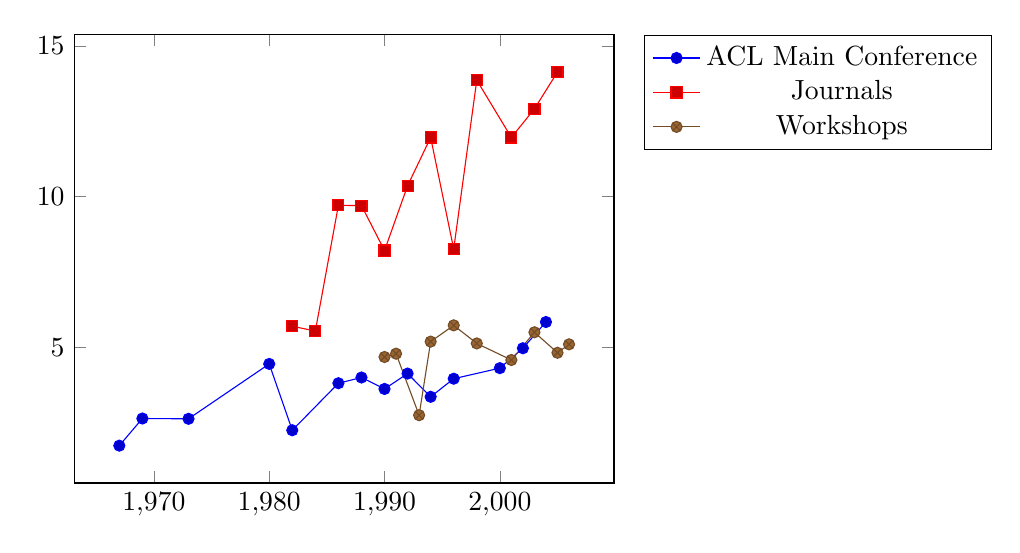
\begin{tikzpicture}
\begin{axis}[
legend style={at={(1.7,1)}, anchor=north east}]
height=9cm,
width=9cm,
grid=major,
xlabel=year,
ylabel=definition per document

\addplot coordinates {
(1967,1.74)
(1969,2.64)
(1973,2.63)
(1980,4.45)
(1982,2.25)
(1986,3.81)
(1988,4.00)
(1990,3.62)
(1992,4.13)
(1994,3.36)
(1996,3.96)
(2000,4.31)
(2002,4.97)
(2004,5.84)
};
\addlegendentry{ACL Main Conference}
\addplot coordinates {
(1982,5.70)
(1984,5.54)
(1986,9.71)
(1988,9.70)
(1990,8.21)
(1992,10.36)
(1994,11.96)
(1996,8.26)
(1998,13.86)
(2001,11.96)
(2003,12.91)
(2005,14.13)
};
\addlegendentry{Journals}
\addplot coordinates {
(1990,4.68)
(1991,4.79)
(1993,2.75)
(1994,5.19)
(1996,5.73)
(1998,5.13)
(2001,4.58)
(2003,5.50)
(2005,4.82)
(2006,5.10)
};
\addlegendentry{Workshops}

\end{axis}
\end{tikzpicture}
\caption{Definitions extracted per document for different types of articles}
\label{plot}
\end{figure}


\chapter{Conclusions and Future Works}

In this work, we revolutionized the task of mining definitions by going beyond just the identification of definition sentence. Instead we propose to identify relevant parts of a sentence that contains a term to be defined, and its definition. Making use of sequence labeling with CRF, we show that we are able to achieve better results over our baseline. Compared to the previous systems based on lexicon-semantic patterns, our system is likely to have a higher recall. It is because our system does not explicitly depend on any word or POS tag patterns and is therefore more robust to different types of definition formulation. 

Though we just made use of some very simple features, the results our system achieved seem very promising, especially its ability to achieve high recalls. We also demonstrated by including shape, dictionary lookup and shallow parsing features we can boost the performance of the system. In this work we also constructed two manually annotated corpora for definition extraction task, with each word token annotated with either ``TERM'', ``DEF'' or ``O''. 

With some adaptations our system can be easily used to extract glossaries or to answer definition questions. We target at producing comparable performance on classifying definition sentences with the state-of-the-art systems, while being able to in addition generate the sequence of labels for each word in the definition sentence. 

\section{Contributions}
\section{Future Work}

\bibliographystyle{socreport}
\bibliography{example}

\appendix
\chapter{Code}

\chapter{Resources}
\section{Hand-crafted Surface Patterns Used by the System}
\textless{}1\textgreater{}  defined (as\textvert{}by) 

\textless{}1\textgreater{} define(s)?  as 

\textless{}1\textgreater{} definition of  

\textless{}1\textgreater{}  a measure of 

\textless{}1\textgreater{}  is (a\textvert{}the)  (that\textvert{}which\textvert{}where\textvert{}if)

\textless{}1\textgreater{}  comprise(s)? 

\textless{}1\textgreater{}  consist(s)? of 

\textless{}1\textgreater{}  denote(s)? 

\textless{}1\textgreater{}  designate(s)? 

\textless{}2\textgreater{}  (is\textvert{}are\textvert{}also) called 

\textless{}2\textgreater{}  (is\textvert{}are\textvert{}also) known as 

\section{Keyphrases Identified by KEA}
For document W00-1219, the KEA system extracts the following keyphrases.
 
Corpus

context dependency

mutual information

extracted compounds

lexicon

parameter settings

extraction of compounds

precision

Chinese Compound

information retrieval

Compound

query

MaxL

new compounds

retrieval

dependency

Large Corpus

parameter

MI

corpora

\end{document}
